\section{Illistrative Examples of Tracking Resource Usage}
\label{sec:example}

We illustrate our technique for static checking of dynamic resources
through two example applications.  First is the surge application in
SOS that uses dynamiclly allocated memory to pass data buffers through
protocol stacks.  Second is the generic base component from TinyOS
that uses swapping of staticlly allocated messages to efficently
implement an interface to receive data messages.  Running on hardware
without memory protection, improper management of either the SOS
buffers or the TinyOS messages can lead to corruption of data or
simply crash the sensor node.

%
% NOTE (ROY): I am not sure that the following figure is doing
% anything other than taking up space.  I will remove it for now.
% 10-18-06
%
%\begin{figure}[t]
%\centering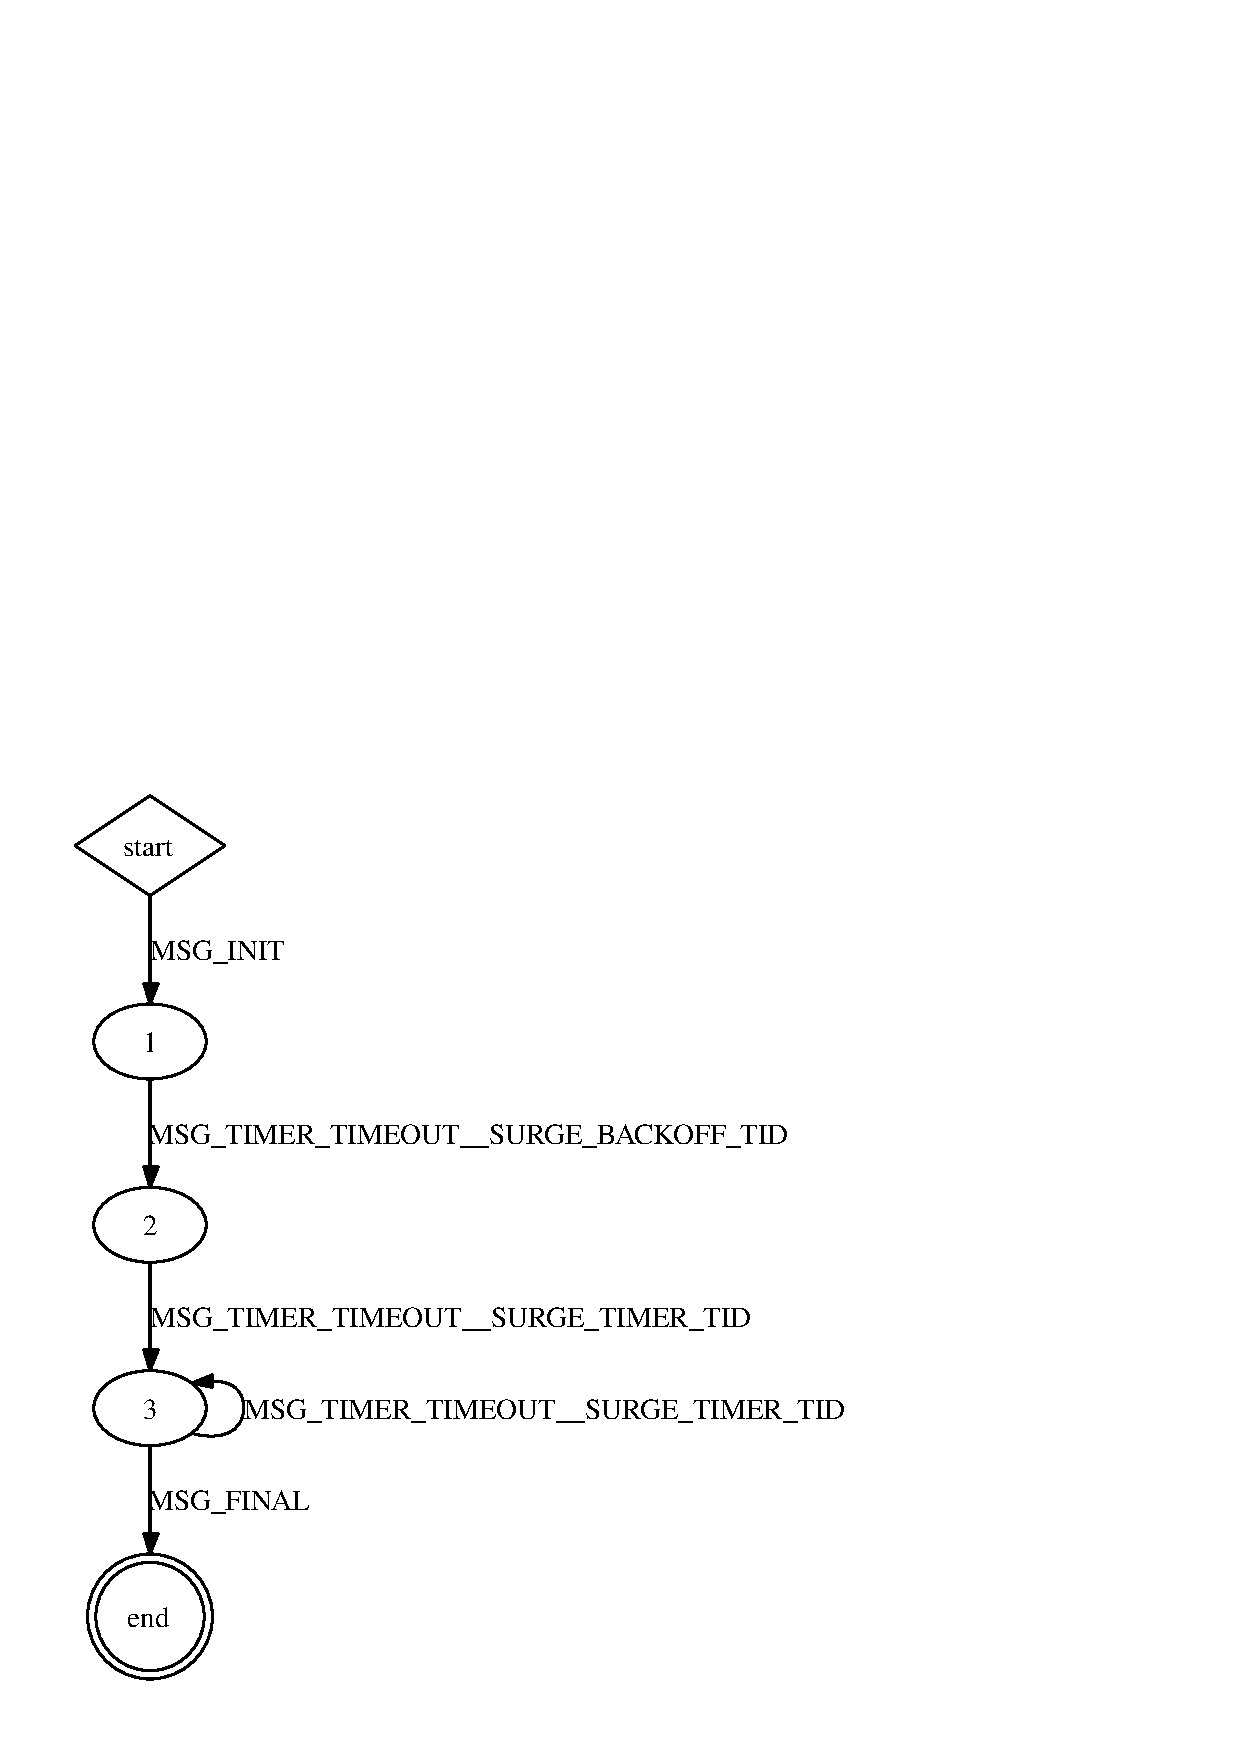
\includegraphics[angle=270,width=4.1in]{surge}
%\caption{{\tt surge} dataflow\label{fig:surge-dataflow}}
%\end{figure}


\subsection{Resource useage in {\tt surge}}

\begin{figure}[t]
\input{surge.c}
\caption{SOS implementation of {\tt surge}\label{fig:surge}}
\end{figure}

Figure~\ref{fig:surge} shows a portion of the SOS module that
implements {\tt surge}, a simple sensor network application that takes
sensor readings and sends the readings over a multihop network to a
base station~\cite{nesC}.  The function {\tt surge\_module} is the
entry point into {\tt surge} for messages from the kernel and from
other modules.  The function takes two arguments: a pointer to the
module's persistent state, which is saved in the kernel, and a pointer
to the current message.  A {\tt switch} statement is used to direct
each message type to an appropriate handler.  The handlers of interest
in this example are for the messages types {\tt MSG\_DATA\_READY} and
{\tt MSG\_TR\_DATA\_PKT}.

A sensor sends the message {\tt MSG\_DATA\_READY} to the surge module
when requested sensor data is ready to be read. The sensor data is
passed as the {\tt data} field of the message, which in general always
contains a message's payload.  Upon receiving this message, the {\tt
surge} message handler allocates a new packet ({\tt ker\_malloc}) to
be sent to the base station and posts a message ({\tt post\_long}) to
the tree-routing module in order to forward the sensor data.  The {\tt
post\_long} call is asynchronous, causing the kernel to package up all
the given arguments into a {\tt Message} structure and to schedule
this message for eventual delivery.

The message {\tt MSG\_TR\_DATA\_PKT} is sent by the tree-routing
module when data is received at the base station node.  Upon receiving
this message, the {\tt surge} message handler confirms that the
current node is the base station.  If so, the message handler forwards
the data to the UART driver via an asynchronous message send ({\tt
post\_net}).

The SOS kernel provides an API for programmers to manage dynamic
memory.  As shown in Figure~\ref{fig:surge}, the {\tt ker\_malloc}
function acts as expected, allocating a new block of memory.  The
kernel also provides a {\tt ker\_free} function for destroying
dynamically allocated memory.  Additionally, ownership of dynamic
memory can be transfered between modules through the messaging
interface provided in SOS.

%
% NOTE (ROY): This is not adding much to the discussion.  10-18-06
%
%In order to provide a simple form of automatic garbage collection for
%dynamically allocated memory, the SOS kernel imposes an {\em
%ownership} model on dynamic memory~\cite{sos}.  Each block of memory
%has a unique owner at any point in time, and the kernel maintains a
%mapping from each block of memory to its owner.  A block's initial
%owner is the module that allocates that block.  For example, the call
%to {\tt ker\_malloc} sets the {\tt surge} module as the initial owner
%of the newly allocated block.  When a module is removed from the
%system at run time, the kernel automatically frees all memory owned by
%that module.

Transfer of dynamic memory ownership occures at the end points of a
message.  First, the owner of a block of dynamically allocated memory
can explicitly {\em release} ownership of that block when it is passed
as the payload in a message.  This is accomplished by setting the
\texttt{SOS\_MSG\_RELEASE} flag in the corresponding {\tt post\_*}
call.  For example, the {\tt surge} module releases ownership of the
newly allocated {\tt pkt} upon sending it to the tree-routing module.
Second, a module can acquire ownership of a message's payload, which
is stored in the {\tt data} field, by calling
\texttt{ker\_msg\_take\_data} on an incoming message.  The function
returns a pointer to the message's payload.  For example, if the
current node is the base station, the {\tt surge} module explicitly
takes ownership of the given message's data under the name {\tt
payload}.

There are four release/take scenarios to consider.  If data is both
released by its sender and taken by its receiver, then ownership of
the data is transferred from the sender to the receiver.  If data is
released by its sender but not taken by its receiver, then the kernel
automatically frees the memory after the receiver's message handler
completes.  If data is not released by its sender but is taken by its
receiver, then the sender keeps ownership of the original message and
the receiver gains ownership of a new block of memory containing a
copy of that data.  Finally, if the data is not released by the sender
and not claimed by the receiver, then the sender keeps ownership of
the original message and the receiver has direct access to
``borrowed'' data for a limited period of time.  This last case is not
generally used in SOS due to the synchronization complications that
can result.


\subsection{Resource useage in {\tt GenericBaseM}}

\begin{figure}[t]
\input{surge.c}
\caption{TinyOS implementation of {\tt GenericBaseM recieve
interface}\label{fig:genericbase}}
\end{figure}


Figure~\ref{fig:genericbase} shows a portion of the TinyOS component that
implements the {\tt receive} event handler for {\tt GenericBase}, an
application that uses a sensor node as a bridge between a base station
and the rest of a sensor network.  The {\tt receive} event handler is
passed in a {\tt TOS\_MsgPtr} pointing to the incoming message and a
flag describing where the message source.

% TODO: Start editing here!!!

% base station~\cite{nesC}.  The function {\tt surge\_module} is the
% entry point into {\tt surge} for messages from the kernel and from
% other modules.  The function takes two arguments: a pointer to the
% module's persistent state, which is saved in the kernel, and a pointer
% to the current message.  A {\tt switch} statement is used to direct
% each message type to an appropriate handler.  The handlers of interest
% in this example are for the messages types {\tt MSG\_DATA\_READY} and
% {\tt MSG\_TR\_DATA\_PKT}.
% 
% A sensor sends the message {\tt MSG\_DATA\_READY} to the surge module
% when requested sensor data is ready to be read. The sensor data is
% passed as the {\tt data} field of the message, which in general always
% contains a message's payload.  Upon receiving this message, the {\tt
% surge} message handler allocates a new packet ({\tt ker\_malloc}) to
% be sent to the base station and posts a message ({\tt post\_long}) to
% the tree-routing module in order to forward the sensor data.  The {\tt
% post\_long} call is asynchronous, causing the kernel to package up all
% the given arguments into a {\tt Message} structure and to schedule
% this message for eventual delivery.
% 
% The message {\tt MSG\_TR\_DATA\_PKT} is sent by the tree-routing
% module when data is received at the base station node.  Upon receiving
% this message, the {\tt surge} message handler confirms that the
% current node is the base station.  If so, the message handler forwards
% the data to the UART driver via an asynchronous message send ({\tt
% post\_net}).
% 
% The SOS kernel provides an API for programmers to manage dynamic
% memory.  As shown in Figure~\ref{fig:surge}, the {\tt ker\_malloc}
% function acts as expected, allocating a new block of memory.  The
% kernel also provides a {\tt ker\_free} function for destroying
% dynamically allocated memory.  Additionally, ownership of dynamic
% memory can be transfered between modules through the messaging
% interface provided in SOS.
% 
% Transfer of dynamic memory ownership occures at the end points of a
% message.  First, the owner of a block of dynamically allocated memory
% can explicitly {\em release} ownership of that block when it is passed
% as the payload in a message.  This is accomplished by setting the
% \texttt{SOS\_MSG\_RELEASE} flag in the corresponding {\tt post\_*}
% call.  For example, the {\tt surge} module releases ownership of the
% newly allocated {\tt pkt} upon sending it to the tree-routing module.
% Second, a module can acquire ownership of a message's payload, which
% is stored in the {\tt data} field, by calling
% \texttt{ker\_msg\_take\_data} on an incoming message.  The function
% returns a pointer to the message's payload.  For example, if the
% current node is the base station, the {\tt surge} module explicitly
% takes ownership of the given message's data under the name {\tt
% payload}.
% 
% There are four release/take scenarios to consider.  If data is both
% released by its sender and taken by its receiver, then ownership of
% the data is transferred from the sender to the receiver.  If data is
% released by its sender but not taken by its receiver, then the kernel
% automatically frees the memory after the receiver's message handler
% completes.  If data is not released by its sender but is taken by its
% receiver, then the sender keeps ownership of the original message and
% the receiver gains ownership of a new block of memory containing a
% copy of that data.  Finally, if the data is not released by the sender
% and not claimed by the receiver, then the sender keeps ownership of
% the original message and the receiver has direct access to
% ``borrowed'' data for a limited period of time.  This last case is not
% generally used in SOS due to the synchronization complications that
% can result.
% 



%%%%%%%%%%%%%%%%%%%%%%%%%%%%%%%%%%%%%%%%%%%%%%%%%%%%%%%%%%%%

\subsection{Static Ownership Checking}

SOS's original concept of ownership as described above
provides a simple form of
garbage collection at run time.
While this can help
reduce the complexity of managing
dynamic memory, it is not sufficient to
prevent memory errors such as dangling pointers and memory leaks.
For example, nothing prevents a module from freeing some memory while
another module (or even the same module) still has a pointer to that
memory.  If that pointer is ever accessed later, an invalid dereference
will result.  Further, garbage collection introduces the potential for
more dangling pointer errors, since the removal of a module implicitly
frees the memory it owns, even if other modules have pointers to that
memory.

%% The basic problem is that SOS's intuitive concept of ownership is
%% not enforced.  There is no guarantee that
%% a program's ownership directives and
%% annotations are consistent with the rest of the program.  Further,
%% there is no explicit notion of what it means to be consistent, namely the
%% rights and responsibilities of owners and non-owners with respect to
%% dynamic memory.  Instead, the burden is on the programmer to ensure
%% that the implicit ownership protocol is properly respected.

In this work, we augment SOS's ownership directives to
provide a protocol governing
memory management that is sufficient to ensure the absence of
memory errors.
Our protocol makes explicit a common programming idiom in
sensor-network systems, whereby data is rarely shared but instead
follows a producer/consumer model.
We have built a tool that checks for violations of this protocol on
each SOS module at compile time.

Informally, the rules of the protocol can be stated as
follows:
\begin{itemize}

\item A module may only manipulate the memory that it owns.

\item A module that takes ownership of a block of memory (either
  through {\tt ker\_malloc} or {\tt ker\_msg\_take\_data}) must either
  free that memory, release it, or store it in the module's
  persistent state.

\item A module may only free or release memory that it owns.  After a module
  frees or releases memory, it may not access or update that memory.
\end{itemize}
Because only the owner can manipulate or free its
memory, dangling pointers are avoided.  Because all memory must be
either freed, released or persistently stored by its owner,
memory leaks are avoided.


\subsection{{\tt surge} Revisited}

Our tool is able to validate at compile time that the
{\tt surge} module properly obeys the ownership protocol.
The {\tt MSG\_DATA\_RDY} message handler
allocates {\tt pkt} and takes
ownership. This pointer is then dereferenced in order to provide the
sensor data
to be sent up the routing tree.
This pointer manipulation is safe since the module has ownership.
The module then
releases ownership by posting {\tt pkt} to the tree routing module
using the {\tt SOS\_MSG\_RELEASE} tag.  After this release, the
module does not access
{\tt pkt} again and does not store it, ensuring that access to the
pointer is indeed released. 

The handler for {\tt MSG\_TR\_DATA\_PKT} also conforms to the
protocol.   When the current
node is the base station, the handler explicitly acquires ownership of
the message's data
using {\tt ker\_msg\_take\_data}.  This allows the module to
manipulate the data and to pass it to
the UART.  The {\tt post\_net} call
explicitly releases the data, fulfilling the module's obligation to
that data.   After the release, the data
is no longer accessed or stored.

While the {\tt surge} code is correct, small changes to the code can
easily cause problems to occur at run time, and our static checker
catches these potential errors.  For example, suppose the handler for
{\tt MSG\_DATA\_READY} did not release ownership of {\tt pkt} by setting the 
{\tt SOS\_MSG\_RELEASE} flag in the call to {\tt post\_long}.
In that case, the module would leak the memory allocated for {\tt pkt}.
Indeed, our checker flags this
modified version of the code as erroneous, since {\tt surge} would not be
freeing, releasing, or storing the data for which it has taken ownership.

\subsection{Function Attributes}

%% The next section details the way in which our tool conservatively
%% ensures at compile time that SOS modules obey this protocol.  The
%% heart of the checker is a suite of dataflow analyses that statically
%% approximate the dynamic ownership relationships.  
%% So far, we have described the analysis for the {\em intra-procedural case},
%% i.e., when there are no function calls.
Our analysis is {\em modular}:  
each function in a module is analyzed in isolation.  To make checking
of a function body precise in the presence of calls to other
functions, we employ
{\em ownership attributes} for function headers that capture the memory-related
behavior of a called function.
We add two attributes to the SOS API: {\tt sos\_claim} and {\tt sos\_release}.
A formal parameter or return value
that has the {\tt sos\_claim} attribute indicates that the
caller must take ownership of the associated memory after a call.
This annotation, for example, would be used to annotate a function that
wraps a call to {\tt ker\_malloc}, allowing that function's callers to
be properly checked without access to the function's implementation.
Similarly, an {\tt sos\_release} attribute on a formal parameter
%
indicates that ownership of the parameter is transferred from the caller of the
function to the callee.
%indicates that the parameter's contents are either released or freed
%(directly or indirectly) by the function.
%
If a parameter does not have an ownership attribute, memory ownership
is unchanged.
%% Our tool makes use of ownership attributes to precisely check callers
%% of a function.  
Our tool ensures that these attributes are employed wherever 
necessary, when checking the implementation of each function. 
%
%% Attributes do not need to reside in the code.  An annotation configuration
%% file can be used by the checker to insert attributes during analyses.  The
%% annotations in this configuration look like:
%% %
%% \begin{footnotesize}
%% \begin{verbatim}
%% add annotations "ker_malloc" [Some "sos_claim"; None; None];
%% \end{verbatim}
%% \end{footnotesize}
%% %
%% specifying that the {\tt sos\_claim} attribute should be added to the 
%% data returned by {\tt ker\_malloc} and that the two formal parameters need
%% no additional ownership attributes.  Our tool assumes that functions not described in
%% the annotation configuration need no other attributes added to them.  
In practice, we have found that a small set of annotations
is sufficient for precise analysis.
%% to obviate the need for explicit attributes annotations in user code.

\subsection{Generality}

Memory errors in SOS were the original motivation for our work.
Further, the existing ownership directives for dynamic
memory in SOS facilitated the creation of our tool.  However, we stress that
the underlying protocol that we enforce
is completely independent of both SOS and of
memory in particular.  For example, it would be straightforward to
apply our tool to track resources other than memory in SOS, and
we could similarly port our tool to enforce an ownership protocol on
nesC's static buffers rather than
SOS's dynamic memory.

